\documentclass{standalone}

% put this in your preamble
\usepackage{tikz}
\usetikzlibrary{hobby}

\begin{document}

% put this tikzpicture block in your LaTeX document where you want the figure
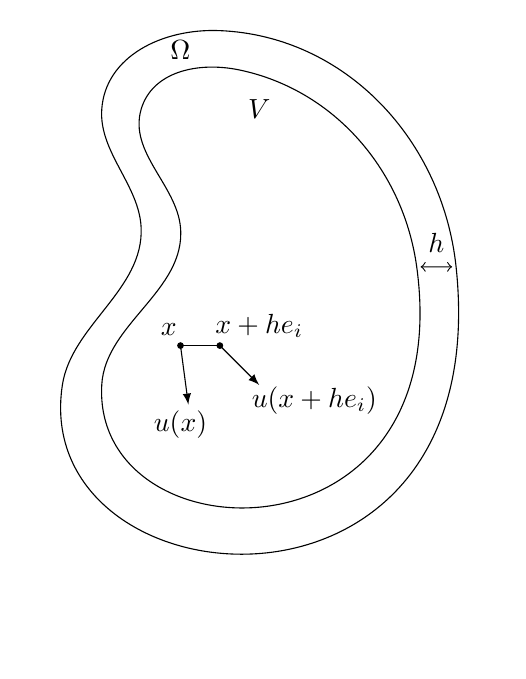
\begin{tikzpicture}[use Hobby shortcut,scale=0.5]
  % \Omega
  \path
  (0,0) coordinate (z0)
  (10,3) coordinate (z1)
  (4,9) coordinate (z2)
  (1,7) coordinate (z3)
  (2,4) coordinate (z4);
  \draw[closed] (z0) .. (z1) .. (z2) .. (z3) .. (z4);
  \node at (3,8.5) {$\Omega$};

  % V
  \path
  (1,0) coordinate (v0)
  (9,3) coordinate (v1)
  (4.5,8) coordinate (v2)
  (2,7) coordinate (v3)
  (3,4) coordinate (v4);
  \draw[closed] (v0) .. (v1) .. (v2) .. (v3) .. (v4);
  \node at (5,7) {$V$};

  % h segment
  \draw[<->] (9.1,3) node[xshift=2mm,yshift=3mm] {$h$} .. (9.9,3);

  % differences segment
  \filldraw (3,1) circle (2pt) node[xshift=-1.5mm,yshift=2mm] {$x$};
  \filldraw (4,1) circle (2pt) node[xshift=5mm,yshift=2.5mm] {$x+he_i$};
  \draw (3,1) -- (4,1);
  \draw[-latex] (3,1) node[xshift=0mm,yshift=-10mm] {$u(x)$} -- +(0.2,-1.5);
  \draw[-latex] (4,1) node[xshift=12mm,yshift=-7mm] {$u(x+he_i)$} -- +(1,-1);

\end{tikzpicture}

\end{document}
